\documentclass{beamer}

\mode<presentation>
{
  \usetheme{Montpellier}
  \usecolortheme{beaver}
  \setbeamercovered{transparent}
  
}

\usepackage[english]{babel}
\usepackage[latin1]{inputenc}
\usepackage{times}
\usepackage[T1]{fontenc} 

% Or whatever. Note that the encoding and the font should match. If T1
% does not look nice, try deleting the line with the fontenc.
\usepackage{amsmath}
\newcommand{\linespace}{\vskip 0.25cm}

\definecolor{MyForestGreen}{rgb}{0,0.7,0} 
\newcommand{\tableemph}[1]{{#1}}
\newcommand{\tablewin}[1]{\tableemph{#1}}
\newcommand{\tablemid}[1]{\tableemph{#1}}
\newcommand{\tablelose}[1]{\tableemph{#1}}
\setbeamertemplate{navigation symbols}{}

\definecolor{MyLightGray}{rgb}{0.6,0.6,0.6}
\newcommand{\tabletie}[1]{\color{MyLightGray} {#1}}

% The text in square brackets is the short version of your title and will be used in the
% header/footer depending on your theme.
\title[Thermal Interaction In SAR]{Thermal Interaction \& \\ 3D Data Visualization}

% Sub-titles are optional - uncomment and edit the next line if you want one.
% \subtitle{Why does sub-tree crossover work?} 

% The text in square brackets is the short version of your name(s) and will be used in the
% header/footer depending on your theme.
\author[YaDeau]{Justin Brennen YaDeau}

% The text in square brackets is the short version of your institution and will be used in the
% header/footer depending on your theme.
\institute[U of Minn, Morris]
{
  Division of Science and Mathematics \\
  University of Minnesota, Morris \\
  Morris, Minnesota, USA
}

% The text in square brackets is the short version of the date if you need that.
\date[December '15] % (optional)
{5 December 2015}

% Delete this, if you do not want the table of contents to pop up at
% the beginning of each subsection:
\AtBeginSection[]
{
  \begin{frame}<beamer>
    \frametitle{Outline}
    \tableofcontents[currentsection, hideothersubsections]
  \end{frame}
}

\begin{document}

\begin{frame}
  \titlepage
\end{frame}

% For a 20-25 minute senior seminar talk you probably want something like:
% - Two or three major sections (other than the summary).
% - At *most* three subsections per section.
% - Talk about 30s to 2min per frame. So there should probably be between
%   15 and 30 frames, all told.

\section*{Overview}

\subsection*{Thermal Interaction \& 3D Data Visualization}
\begin{frame}
	\begin{itemize}
		\item What would thermal interaction \& 3D data visualization look like? 
	\end{itemize}
\end{frame}

\subsection*{Outline}
\begin{frame}
  \frametitle{Outline}
  \tableofcontents[hideallsubsections]
\end{frame}

\section{Background}

\subsection{Virtual Reality}
\begin{frame}
	\frametitle{Virtual Reality}
	\begin{columns}
    \begin{column}{0.4\textwidth}
	\begin{itemize}
		\item Completely Virtual
		\item Oculus Rift
	\end{itemize}
	\end{column}
	\begin{column}{0.4\textwidth}
	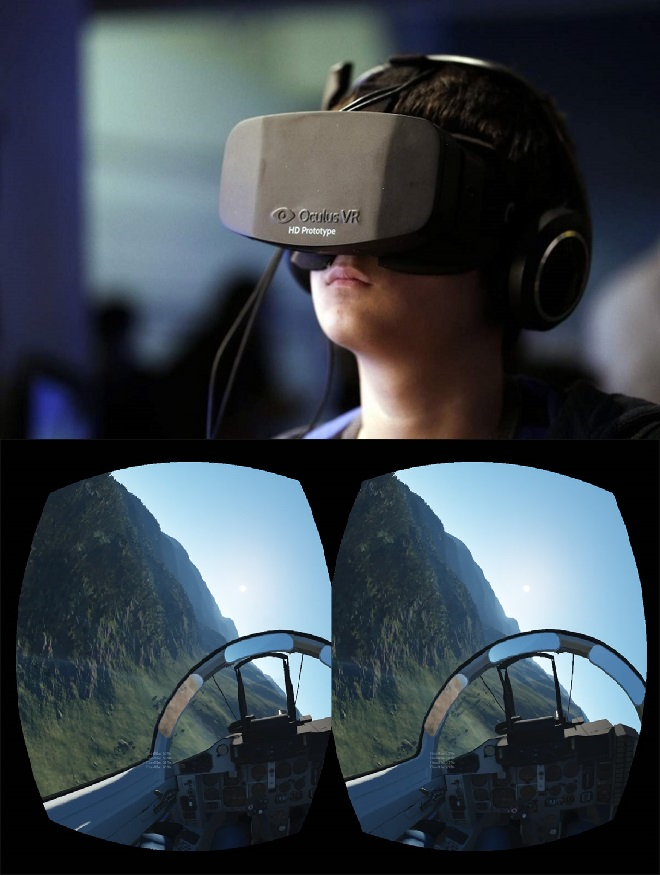
\includegraphics[width=\textwidth]{images/OculusRift}
	
	\tiny Top - http://appleinsider.com/articles/15/05/15/mac-development-for-oculus-rift-vr-headset-paused-ahead-of-early-2016-windows-launch
	Bottom - http://www.theriftarcade.com/outerra-preview-fly-planes-drive-buses-and-steer-boats/
	\end{column}
    \end{columns}
\end{frame}

\subsection{Augmented Reality}
\begin{frame}
	\frametitle{Augmented Reality}
	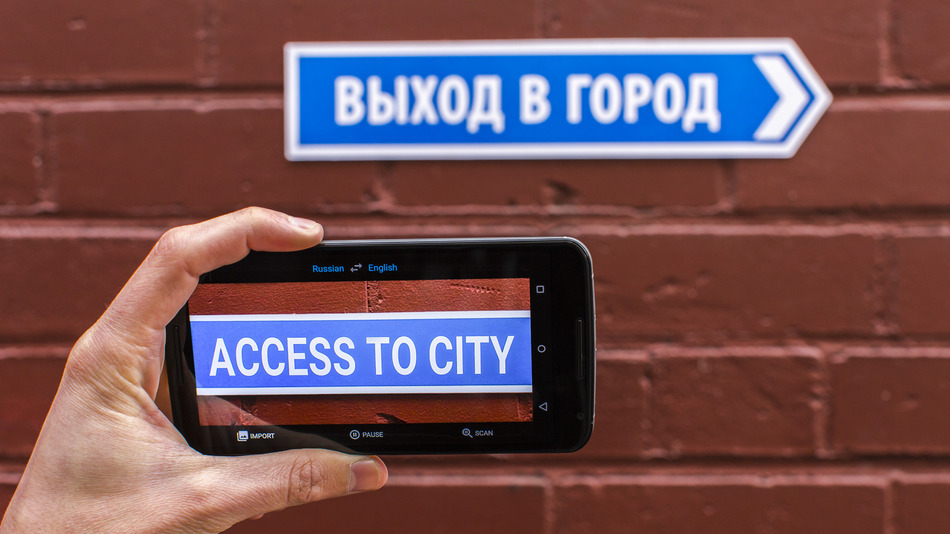
\includegraphics[width=\textwidth]{images/google-translate}
	\begin{center}
	\Tiny http://www.emergingedtech.com/2015/08/translate-language-text-on-the-fly-using-phone-google-translate-app/
	\end{center}
\end{frame}

\subsection{Spatial Augmented Reality}
\begin{frame}
	\frametitle{Spatial Augmented Reality}
	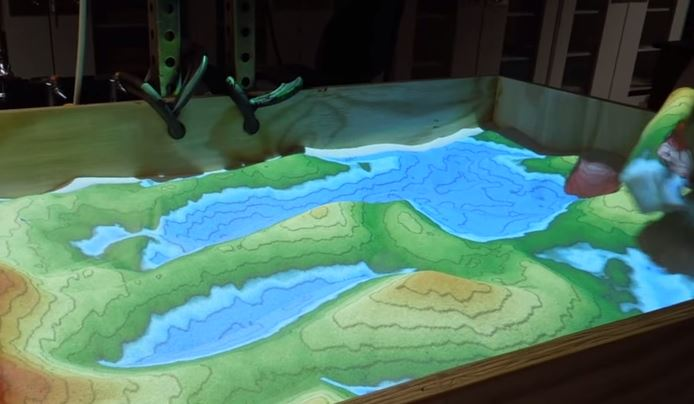
\includegraphics[width=\textwidth]{images/Augmented-Reality-Sandbox}
	\begin{center}
	\tiny http://peanutchuck.com/augmented-reality-sandbox/
	\end{center}
\end{frame}

\subsection{6DOF}
\begin{frame}
	\frametitle{6DOF}
	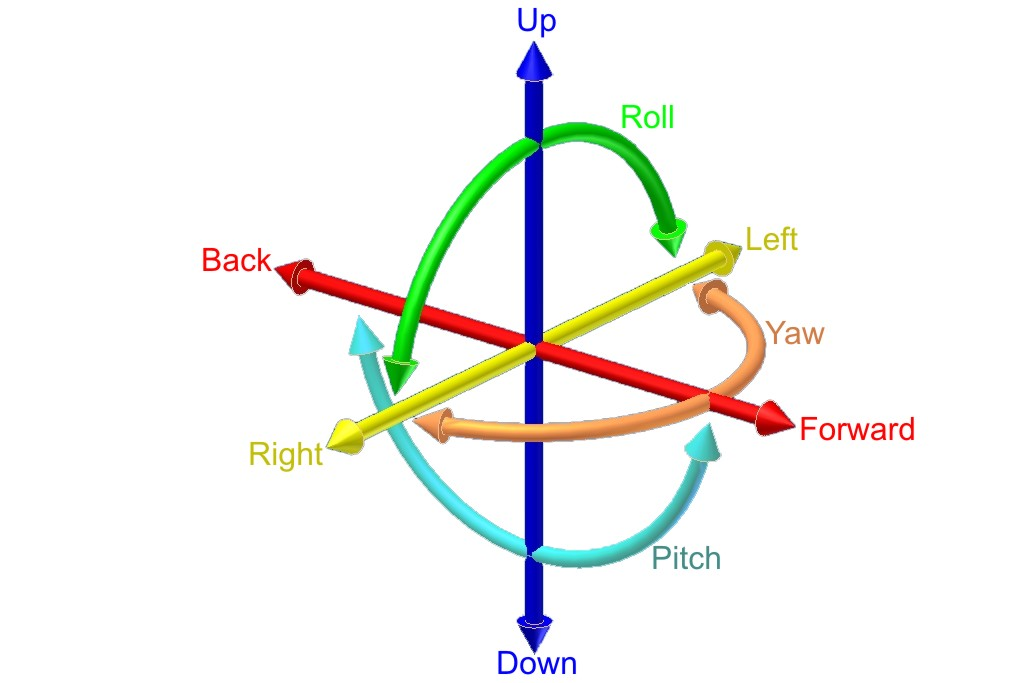
\includegraphics[width=10cm]{../Sample_paper/images/6DOF_en}
	\begin{center}
	\cite{6DOF}
	\end{center}
\end{frame}

\section[Mobile Thermal Interaction]{Thermal interaction with mobile devices}

\subsection{Interacting with Objects}
\begin{frame}
\frametitle{Interactions with Objects}	
	\begin{columns}
    \begin{column}{0.7\textwidth}
	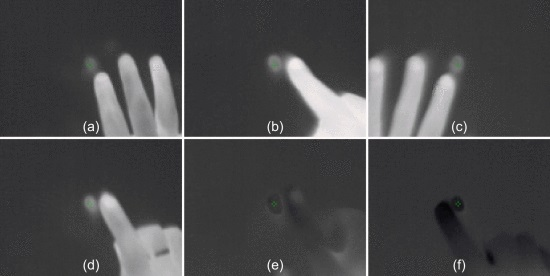
\includegraphics[width=\textwidth]{images/Thermal}
	
	\cite{Thermal}
	\end{column}
	\begin{column}{0.4\textwidth}
	\begin{itemize}
		\item Interactions leave thermal impressions on the object
		\item Using these impressions to interact with a device in a new way 
	\end{itemize}	
	\end{column}
    \end{columns}
\end{frame}

\subsection{Hardware}
\begin{frame}
\frametitle{Hardware}	
	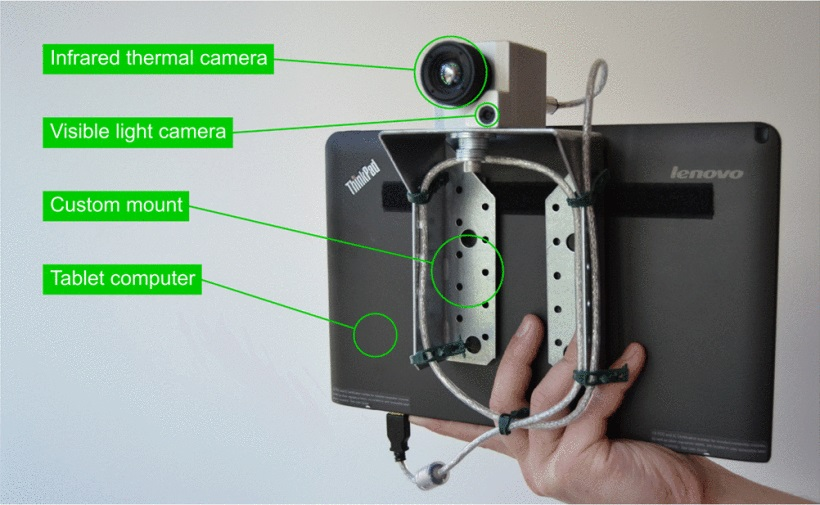
\includegraphics[width=\textwidth]{../Sample_paper/images/Hardware2}
	\begin{center}
	\cite{Thermal}
	\end{center}
\end{frame}

\subsection{Thermal Detection}
\begin{frame}
\frametitle{Thermal Detection}
	\begin{itemize}
		\item Assumes a controlled environment
		\item Object-only, hand-only, obstruction-by-hand, and touch-by-hand
		\item Using the OpenCV SimpleBlobDetector
	\end{itemize}
\end{frame}

\begin{frame}
\frametitle{OpenCV SimpleBlobDetector}
\begin{center}
	\(
\begin{matrix} \\
 t_{1}=(1-{1\over 16})t_{ min}+{1\over 16}t_{ max} & t_{2}=(1-{3\over 8})t_{ min}+{3\over 8}t_{ max}\cr 
 \end{matrix} 
\)
\end{center}
	\begin{itemize}
		\item \(t_{1}\) and \(t_{2}\) is the expected temperature range of the interaction
		\item With a fixed size range of \(0.32cm^2\) and \(1.54cm^2\)
	\end{itemize}
	\begin{center}
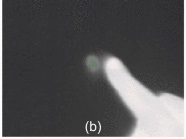
\includegraphics[width=4.5cm]{images/ThermalSnip}

	\cite{Thermal}
\end{center}
\end{frame}

\subsection{Object Tracking}
\begin{frame}	
\frametitle{Object Tracking}
	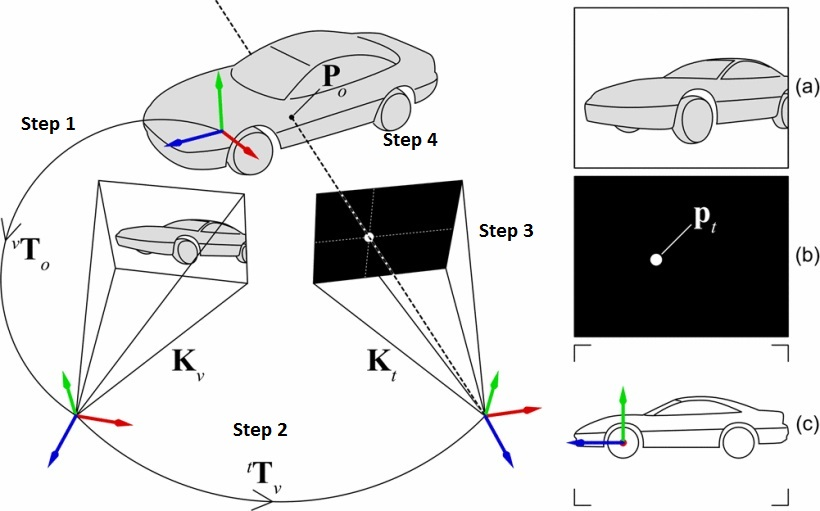
\includegraphics[width=\textwidth]{images/Tracking}
	\begin{center}
	\cite{Thermal}
	\end{center}
\end{frame}

\subsection{Materials Tested}
\begin{frame}	
\frametitle{Materials Tested}
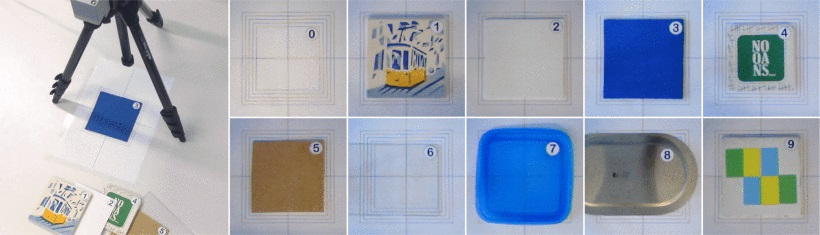
\includegraphics[width=\textwidth]{../Sample_paper/images/ThermalTesting}

Different materials used during the evaluation: (0) paper on a plastic table-top, (1) ceramic, (2) rigid PVC, (3) foam plastic, (4) cardboard, (5) laminated fiber sheet, (6) glass, (7) thin plastic, (8) steel, (9) multi-layer board
\begin{center}
	\cite{Thermal}
	\end{center}
\end{frame}


\subsection{Applications}

\begin{frame}
	\frametitle{Applications}
	Some applications that use thermal imaging with mobile technology 
	\begin{itemize}
		\item "Spray on" graphical user interfaces (GUI)
		\item Augmented floor plans
	\end{itemize}
\end{frame}

\begin{frame}
	\frametitle{"Spray on" GUIs}	
	\begin{columns}
	\begin{column}{0.45\textwidth}
	\begin{itemize}
		\item The screen displays a dial pad, but there is no dial pad on the surface
		\item Looking at the screen to interact with dial pad
		\item Devices without touch screens
	\end{itemize}		
	\end{column}
	\begin{column}{0.55\textwidth}
	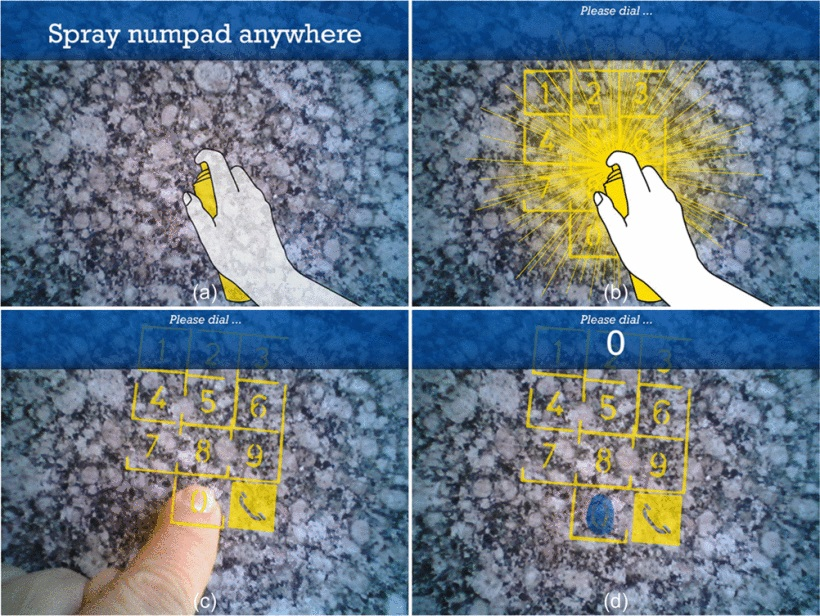
\includegraphics[width=\textwidth]{../Sample_paper/images/numpad}
	
	\cite{3D}
	\end{column}
	\end{columns}
\end{frame}

\begin{frame}
	\frametitle{Augmented Floor Plans}
	\begin{columns}
	\begin{column}{0.45\textwidth}
	\begin{itemize}
		\item Similar interaction, different interface
		\item Using the areas on the map as buttons
	\end{itemize}
	\end{column}
	\begin{column}{0.55\textwidth}
	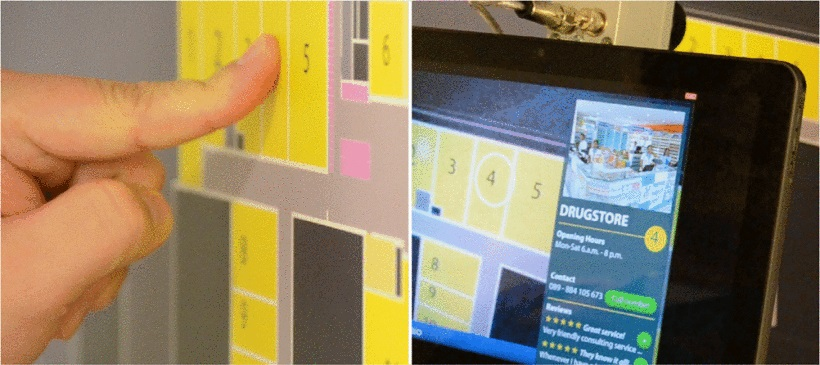
\includegraphics[width=\textwidth]{images/AugmentedFloorPlans}
	
	\cite{3D}
	\end{column}
	\end{columns}	
\end{frame}

\section[Using spatial augmented reality for 3D data visualization]{Using spatial augmented reality for 3D data visualization}

\subsection{Visualizing Data}
\begin{frame}	
\frametitle{Visualizing Data}
	\begin{itemize}
		\item Representing data with images
		\item Examples: weather maps, pie and bar charts, etc
		\item The importance of visualizing data
	\end{itemize}
\end{frame}

\subsection{Applications}
\begin{frame}
\frametitle{Applications}
	Some applications that use spatial augmented reality for 3D data visualization   
	\begin{itemize}
		\item Table-Top
		\item CAVE
	\end{itemize}
\end{frame}

\begin{frame}
\frametitle{Table-Top} 
	\begin{columns}
    \begin{column}{0.9\textwidth}
    \begin{itemize}
		\item Physical object represents the 3D space
		\item The display is a 2D representation of the 3D space
		\item 6DOF trackers
	\end{itemize}
	
	\begin{center}
	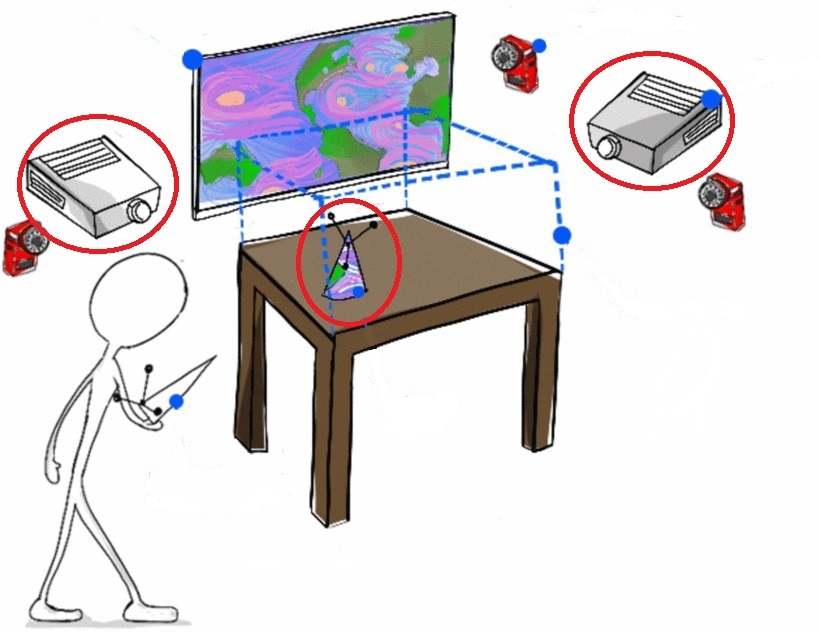
\includegraphics[width=6cm]{images/TabletopPO}
	
	\cite{3D}
	\end{center}
	\end{column}
    \end{columns}
\end{frame}

\begin{frame}
\frametitle{Table-Top} 
	\begin{columns}
    \begin{column}{0.9\textwidth}
    \begin{itemize}
		\item Physical object represents the 3D space
		\item The display is a 2D representation of the 3D space
		\item 6DOF trackers
	\end{itemize}
	
	\begin{center}
	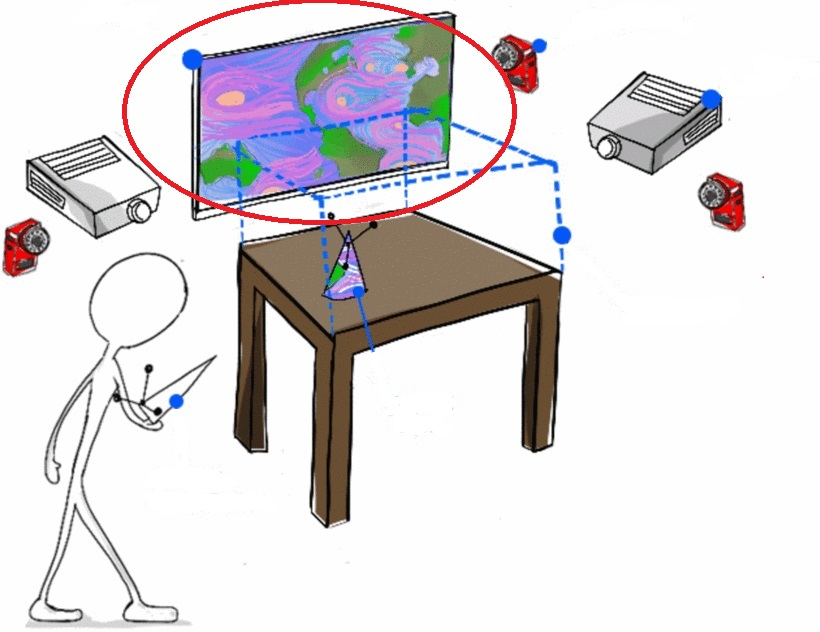
\includegraphics[width=6cm]{images/TabletopDis}
	
	\cite{3D}
	\end{center}
	\end{column}
    \end{columns}
\end{frame}

\begin{frame}
\frametitle{Table-Top} 
	\begin{columns}
    \begin{column}{0.9\textwidth}
    \begin{itemize}
		\item Physical object represents the 3D space
		\item The display is a 2D representation of the 3D space
		\item 6DOF trackers
	\end{itemize}
	
	\begin{center}
	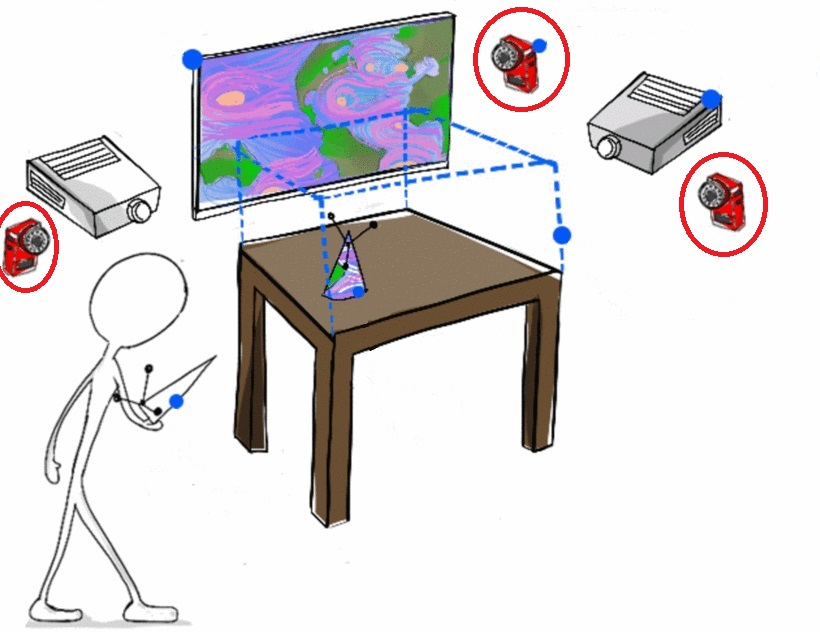
\includegraphics[width=6cm]{images/Tabletop6DOF}
	
	\cite{3D}
	\end{center}
	\end{column}
    \end{columns}
\end{frame}

\begin{frame}
\frametitle{Table-Top} 
	\begin{columns}
    \begin{column}{0.9\textwidth}
    \begin{itemize}
		\item Using a hand held pointing device a user can zoom in or out of the visualization 
		\item Interactions happen inside the virtual volume
	\end{itemize}
	\begin{center}

	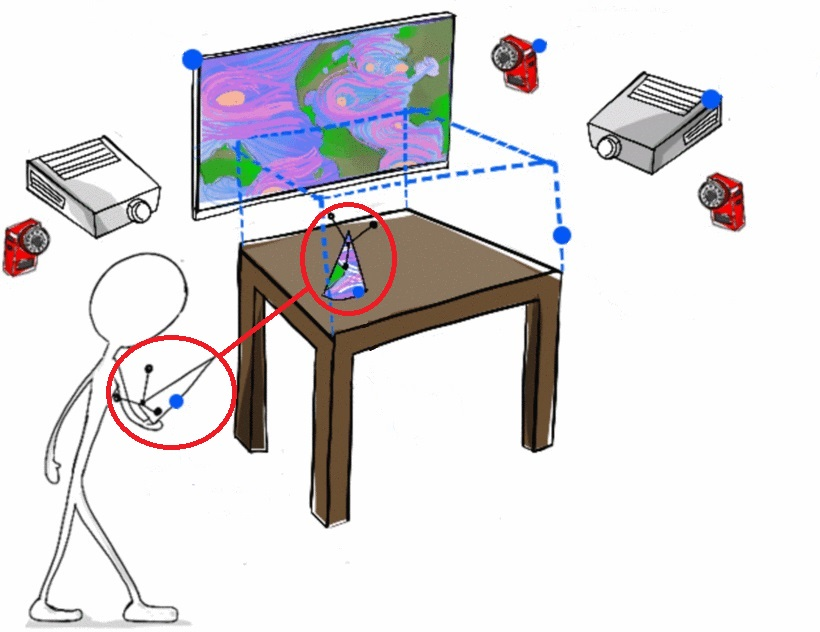
\includegraphics[width=6cm]{images/TabletopZoom}
	
	\cite{3D}
	\end{center}
	\end{column}
    \end{columns}
\end{frame}

\begin{frame}
\frametitle{Table-Top} 
	\begin{columns}
    \begin{column}{0.9\textwidth}
    \begin{itemize}
		\item Using a hand held pointing device a user can zoom in or out of the visualization 
		\item Interactions happen inside the virtual volume
	\end{itemize}
	\begin{center}

	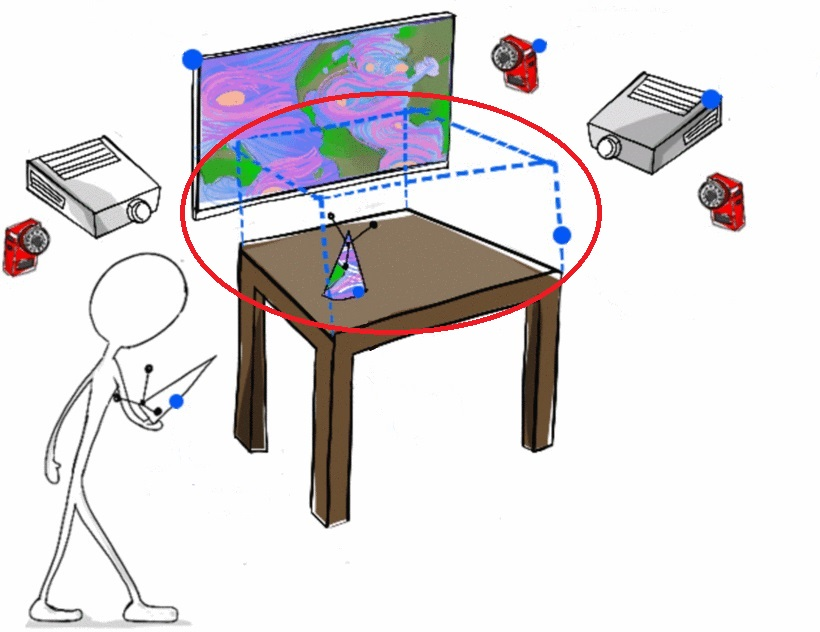
\includegraphics[width=6cm]{images/TabletopVV}
	
	\cite{3D}
	\end{center}
	\end{column}
    \end{columns}
\end{frame}

\begin{frame}
\frametitle{CAVE}
	\begin{columns}
    \begin{column}{0.7\textwidth}
    \begin{itemize}
		\item CAVE - Cave Automatic Virtual Environment 
		\item Larger area than the table-top method
	\end{itemize}
	\begin{center}
	\includegraphics[width=6cm]{../Sample_paper/images/CAVE}
		
	\cite{3D}
	\end{center}
	\end{column}
    \end{columns}
\end{frame}

\begin{frame}
\frametitle{CAVE}
\begin{columns}
    \begin{column}{0.7\textwidth}
    \begin{itemize}
		\item Similar interactions as the table-top method
		\item Increase in collaborators/viewers
	\end{itemize}
		\begin{center}
	\includegraphics[width=6cm]{../Sample_paper/images/CAVE}
		
	\cite{3D}
	\end{center}
	\end{column}
    \end{columns}
\end{frame}

\subsection{Limitations}
\begin{frame}	
\frametitle{Limitations}
    \begin{columns}
    \begin{column}{.8\textwidth}
	\begin{itemize}
		\item Strength of the projectors 
		\item Need for a controlled environment for projectors and 6DOF trackers
		\item Solution
	\end{itemize}
	\end{column}
	\end{columns}
\end{frame}

\section[Conclusions]{Conclusions}
\begin{frame}
\frametitle{Conclusions}
	\begin{itemize}
		\item Utilizing both thermal interaction and 3D data visualization new applications are possible
		\item Examples: education and transportation

	\end{itemize}
\end{frame}

\begin{frame}[allowframebreaks]{Bibliography} 
\bibliographystyle{plainnat}
\bibliography{annotatedBibliography}
\end{frame}

\begin{frame}
	\frametitle{Thanks!}
	
	Thank you for your time and attention!
		
	\linespace
	\linespace
	
	Contact:  
	\begin{itemize}
		\item \texttt{yadea003@morris.umn.edu}
	\end{itemize}
	
	\linespace
	\linespace
	
	\begin{center}
	{\huge Any Questions?}
	\end{center}
\end{frame}

\end{document}


